\documentclass[12pt,a4paper]{article}

%% Package using
\usepackage[utf8]{inputenc}
\usepackage{xeCJK}
\usepackage{graphicx}


%% Document Style
\linespread{1.5}    % 行距    
\setCJKmainfont{NotoSansTC-Regular.otf}   % 中文字型_黑體
\renewcommand{\familydefault}{\sfdefault}   % 英文字型_sans font
\renewcommand\contentsname{目錄}    % TOC標題 : Content -> 目錄
\graphicspath{{./Pic/}}     % 圖片路徑


%% Document Content
\begin{document}

% Title page
\begin{center}
    
    \vspace*{5cm}
    \textbf{\huge Orientation Homework Report}\\   % 粗體+加大
    
    \vspace{1cm}
    {\large 10-bar truss optimization}
    
    \vfill
    {\Large 徐若瑄}
    
    \vspace{1cm}
    {\Large \today}

\end{center}
\newpage

% %----------------Next Page--------------

% \tableofcontents
% \newpage

% %----------------Next Page--------------

% Section 1
\section{問題描述}

    十桿衍架(10-bar truss)由十個長桿件組成並且有6個端點,其中第5、6號端點為固定端,桿件的配置如圖\ref{10-bar truss}所示。
    
    \begin{figure}[h]
        \centering
        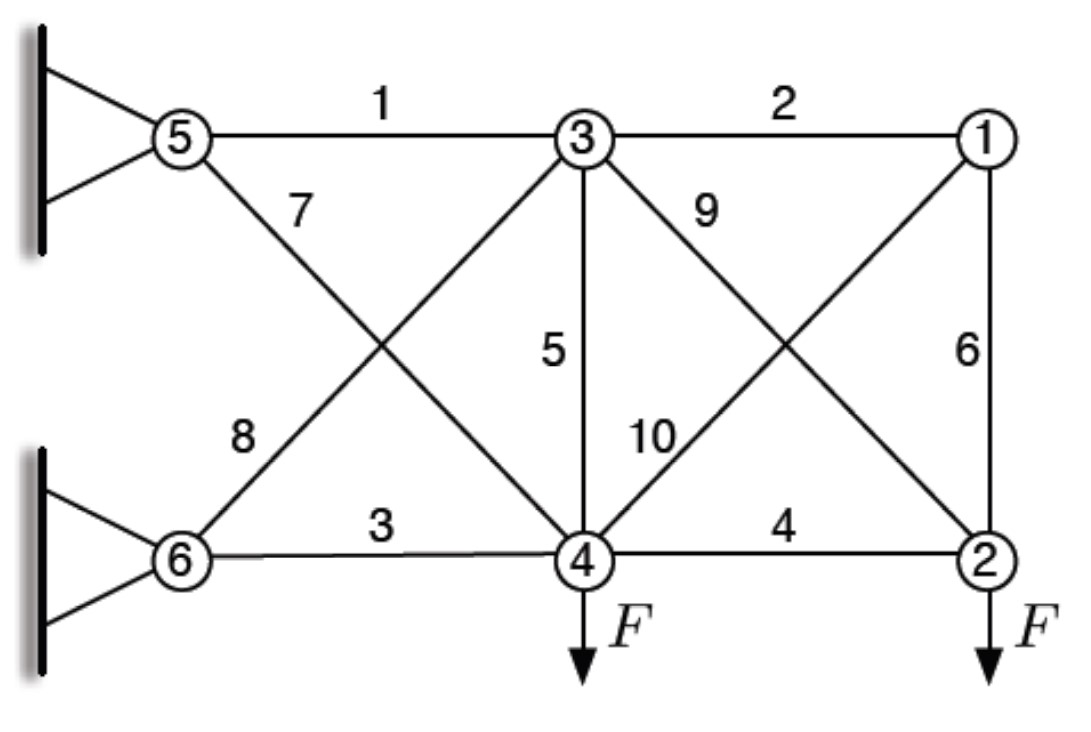
\includegraphics[width=8cm]{10_bar_truss}
        \caption{10-bar truss}
        \label{10-bar truss}
    \end{figure}
    
    所有桿件的截面皆為圓形,桿件1到桿件6的截面半徑同為$r1$且長度為$9.14\  m$;桿件7到桿件8的截面半徑同為$r2$。
    桿件所使用的材料為剛,相關的材料性質有:
    
    \begin{enumerate}
        \item 密度 $\rho = 7860\ kg/m^3$
        \item 楊氏模數(Young's Modulus) $E = 200\ GPa$
        \item 降伏係數(Yield stress) $\sigma_y = 250\ MPa$
    \end{enumerate}
    
    端點4及端點5有一向下的外力$F = 1.0x10^-7\ N$,
    在所有桿件的應力不超過降伏應力且端點2的位移小於$0.02\ m$的條件下,
    求桿件截面半徑$r1$與$r2$的值,使得十桿衍架整體重量為最輕。
    
\newpage
%----------------Next Page--------------

% Section 2
\section{計算方法}
    


\newpage
%----------------Next Page--------------

% Section 3
\section{結論}

\end{document}
